\documentclass[11pt]{article}

\usepackage[margin=1in]{geometry}
\usepackage{amsmath,amssymb,amsthm,mathtools}
\usepackage{booktabs}
\usepackage{enumitem}
\usepackage{algorithm}
\usepackage{algpseudocode}
\usepackage{tikz}
\usetikzlibrary{arrows.meta}

\newcommand{\studentname}{Xilang Chen}
\newcommand{\studentid}{524031910668}

\DeclarePairedDelimiter{\floor}{\lfloor}{\rfloor}
\DeclarePairedDelimiter{\ceil}{\lceil}{\rceil}
\newcommand{\neglit}[1]{\overline{#1}}

\newtheorem*{claim}{Claim}
\newtheorem*{lemma}{Lemma}
\theoremstyle{definition}
\newtheorem*{remark}{Remark}

\setlength{\parindent}{0pt}
\setlength{\parskip}{0.6em}

\tikzset{
  lit/.style={circle, draw, minimum size=8mm, inner sep=0pt, font=\small},
  imp/.style={-{Stealth[length=2.2mm]}, semithick},
}

\title{SE3308 Algorithm Design I --- Assignment 2\\[0.3em]
  \large Exercises 2.14, 2.19, 2.22, 3.7, 3.11, 3.28}
\author{\studentname\ifx\studentid\empty\else\quad\studentid\fi}
\date{}

\begin{document}
\maketitle

Throughout, $\log$ denotes $\log_2$. Graphs are given by adjacency lists, with $n=|V|$ and $m=|E|$.

%======================================================================
\section*{Exercise 2.14}

We assume the elements can be compared (any total order works, e.g.\ the order of their binary encodings).

\textbf{Algorithm.} Sort the array with mergesort, then scan it once and keep an element only if it differs from
its predecessor.

\begin{algorithm}[H]
\caption{Removing duplicates}
\begin{algorithmic}[1]
\Function{RemoveDuplicates}{$A[1..n]$}
  \State $A\gets\Call{MergeSort}{A}$
  \State $B\gets$ empty list
  \For{$i\gets1$ \textbf{to} $n$}
    \If{$i=1$ \textbf{or} $A[i]\neq A[i-1]$}
      \State append $A[i]$ to $B$
    \EndIf
  \EndFor
  \State \Return $B$
\EndFunction
\end{algorithmic}
\end{algorithm}

\textbf{Correctness.} After sorting, equal elements are contiguous: if $A[i]=A[j]$ with $i<j$, then for every
$i\le l\le j$ we have $A[i]\le A[l]\le A[j]=A[i]$, so $A[l]=A[i]$. Hence the sorted array consists of maximal
runs, each run containing all copies of one distinct value. The scan appends exactly the first element of each run
(the first element of a run either is $A[1]$ or differs from its predecessor, which belongs to the previous run;
every other element of a run equals its predecessor). Therefore $B$ contains every distinct value of the input
exactly once.

\textbf{Running time.} Mergesort takes $O(n\log n)$ and the scan takes $O(n)$, so the total is
$\boxed{O(n\log n)}$.

\begin{remark}
If the original order of the surviving elements must be kept, sort the pairs $(A[i],i)$ lexicographically instead,
keep the first pair of each run (it carries the smallest index of that value), and finally sort the survivors by
index. This is still $O(n\log n)$.
\end{remark}

%======================================================================
\section*{Exercise 2.19}

Recall that \textsc{merge} combines two sorted arrays of total length $L$ in $O(L)$ time.

\textbf{(a)} After merging the first $i$ arrays we hold a sorted array of $in$ elements; merging in the
$(i+1)$-st array costs $\Theta(in+n)=\Theta((i+1)n)$. The total time is
\[
  \sum_{i=1}^{k-1}\Theta\bigl((i+1)n\bigr)
  =\Theta\Bigl(n\sum_{j=2}^{k}j\Bigr)
  =\Theta\Bigl(n\Bigl(\tfrac{k(k+1)}{2}-1\Bigr)\Bigr)
  =\boxed{\Theta(k^2n)}.
\]

\textbf{(b)} Divide and conquer: split the $k$ arrays into two groups of $\ceil{k/2}$ and $\floor{k/2}$ arrays,
merge each group recursively, and merge the two results.

\begin{algorithm}[H]
\caption{$k$-way merge}
\begin{algorithmic}[1]
\Function{MultiMerge}{$A_1,\dots,A_k$}
  \If{$k=1$} \State \Return $A_1$ \EndIf
  \State $h\gets\ceil{k/2}$
  \State $L\gets\Call{MultiMerge}{A_1,\dots,A_h}$
  \State $R\gets\Call{MultiMerge}{A_{h+1},\dots,A_k}$
  \State \Return $\Call{Merge}{L,R}$
\EndFunction
\end{algorithmic}
\end{algorithm}

\emph{Correctness} follows by induction on $k$: for $k=1$ the single array is already sorted; for $k\ge2$, by
induction $L$ and $R$ are sorted and together contain all $kn$ elements, and \textsc{merge} of two sorted arrays
is sorted.

\emph{Running time.} Let $T(k)$ be the time for $k$ arrays of $n$ elements each. The top-level merge handles
$kn$ elements, so
\[
  T(k)=T(\ceil{k/2})+T(\floor{k/2})+O(kn),\qquad T(1)=O(1).
\]
In the recursion tree, the subproblems on any one level involve disjoint groups of the original arrays, so the
merges on that level handle at most $kn$ elements in total and cost $O(kn)$. Group sizes halve (rounding up) at each
level, so there are $\ceil{\log k}$ levels with merges. Hence
\[
  T(k)=\boxed{O(kn\log k)},
\]
an improvement by a factor of $k/\log k$ over part (a).

%======================================================================
\section*{Exercise 2.22}

Let the sorted lists be $A[1..m]$ and $B[1..n]$, stored as arrays (constant-time access by index), and let
$1\le k\le m+n$. For convenience set $A[0]=B[0]=-\infty$ and $A[m+1]=B[n+1]=+\infty$.

\textbf{Idea.} The $k$ smallest elements of the union consist of a prefix $A[1..i]$ of $A$ and a prefix
$B[1..j]$ of $B$ with $i+j=k$. We binary-search for the right $i$. The feasible range is
\[
  \ell=\max(0,\,k-n)\ \le\ i\ \le\ h=\min(k,\,m),
\]
because $0\le i\le m$ and $0\le j=k-i\le n$. For $i$ in this range define the predicate
\[
  P(i):\quad i=\ell\ \ \text{or}\ \ A[i]\le B[k-i+1].
\]

\begin{algorithm}[H]
\caption{$k$-th smallest element of $A\cup B$}
\begin{algorithmic}[1]
\Function{Select2}{$A[1..m],B[1..n],k$}
  \State $\ell\gets\max(0,k-n)$;\quad $h\gets\min(k,m)$
  \While{$\ell<h$} \Comment{invariant: $P(\ell)$ holds and the largest $i$ with $P(i)$ lies in $[\ell,h]$}
    \State $i\gets\ceil{(\ell+h)/2}$ \Comment{$\ell<i\le h$}
    \If{$A[i]\le B[k-i+1]$}
      \State $\ell\gets i$
    \Else
      \State $h\gets i-1$
    \EndIf
  \EndWhile
  \State $i\gets\ell$;\quad $j\gets k-i$
  \State \Return $\max(A[i],B[j])$
\EndFunction
\end{algorithmic}
\end{algorithm}

Inside the loop $\ell<i\le h$ implies $1\le i\le m$ and $1\le k-i+1\le n$ (since $i\ge \ell+1\ge k-n+1$ and
$i\le k$), so both indices refer to real elements.

\textbf{Correctness.}
\emph{Monotonicity.} As $i$ grows, $A[i]$ does not decrease and $B[k-i+1]$ does not increase. So if
$A[i]\le B[k-i+1]$ fails for some $i$, it fails for all larger $i$. Hence $P$ is true on an initial segment
$[\ell,i^*]$ of the range and false afterwards, and the binary search returns $i=i^*$, the largest $i$ with $P(i)$
(each step keeps $P(\ell)$ true and discards only indices where $P$ is false).

\emph{The split is correct.} Let $i=i^*$ and $j=k-i$. We claim
\[
  \text{(1) } A[i]\le B[j+1] \qquad\text{and}\qquad \text{(2) } B[j]\le A[i+1].
\]
For (1): if $i>\ell$ this is $P(i)$. If $i=\ell=0$ then $A[0]=-\infty$; if $i=\ell=k-n$ then $j=n$ and
$B[n+1]=+\infty$.
For (2): if $i<h$, then $P(i+1)$ is false, i.e.\ $A[i+1]>B[k-i]=B[j]$. If $i=h=m$ then $A[m+1]=+\infty$; if
$i=h=k$ then $j=0$ and $B[0]=-\infty$.

Now let $X=A[1..i]\cup B[1..j]$ ($k$ elements) and $Y=A[i+1..m]\cup B[j+1..n]$. Every element of $X$ is at most
every element of $Y$: within one array this is sortedness, and across arrays
$A[1..i]\le A[i]\le B[j+1]\le B[j+1..n]$ by (1) and $B[1..j]\le B[j]\le A[i+1]\le A[i+1..m]$ by (2).
Therefore $X$ is a set of $k$ smallest elements of the union, and the $k$-th smallest element is the maximum of
$X$, which is $\max(A[i],B[j])$ (at least one of $i,j$ is positive because $k\ge1$, so the maximum is finite).

\textbf{Running time.} Each iteration does $O(1)$ work and roughly halves $h-\ell$, which is initially at most
$\min(m,n,k)$. Hence the time is
\[
  O\bigl(1+\log\min(m,n)\bigr)\subseteq \boxed{O(\log m+\log n)}.
\]

%======================================================================
\section*{Exercise 3.7}

\textbf{(a)} Run DFS and give each newly discovered vertex the color opposite to its parent's. The graph is
bipartite iff no edge joins two vertices of the same color.

\begin{algorithm}[H]
\caption{Testing bipartiteness}
\begin{algorithmic}[1]
\Function{Bipartite}{$G=(V,E)$}
  \For{each $v\in V$} \State $\mathit{color}(v)\gets\textsc{nil}$ \EndFor
  \For{each $s\in V$}
    \If{$\mathit{color}(s)=\textsc{nil}$}
      \State $\mathit{color}(s)\gets0$;\quad $\Call{Explore}{s}$
    \EndIf
  \EndFor
  \State \Return \textsc{yes} \Comment{$V_1=\{v:\mathit{color}(v)=0\}$, $V_2=\{v:\mathit{color}(v)=1\}$}
\EndFunction
\Statex
\Procedure{Explore}{$u$}
  \For{each edge $\{u,v\}\in E$}
    \If{$\mathit{color}(v)=\textsc{nil}$}
      \State $\mathit{color}(v)\gets1-\mathit{color}(u)$;\quad $\Call{Explore}{v}$
    \ElsIf{$\mathit{color}(v)=\mathit{color}(u)$}
      \State halt and \Return \textsc{no}
    \EndIf
  \EndFor
\EndProcedure
\end{algorithmic}
\end{algorithm}

\emph{Running time.} This is DFS with $O(1)$ extra work per vertex and per adjacency-list entry: $O(n+m)$.

\emph{Correctness.}
If the algorithm answers \textsc{yes}, every vertex is colored, and every edge $\{u,v\}$ was examined from $u$ when
$\textsc{Explore}(u)$ ran, at which point $v$ was either colored now with the opposite color or already colored
and checked to differ. So every edge joins $V_1$ and $V_2$: the graph is bipartite.

If the algorithm answers \textsc{no}, it found an edge $\{u,v\}$ with $\mathit{color}(u)=\mathit{color}(v)$, and
$u,v$ lie in the same DFS tree $T$ (rooted at some $s$). Suppose for contradiction that $G$ had a bipartition,
i.e.\ a function $c:V\to\{0,1\}$ with $c(x)\neq c(y)$ for every edge $\{x,y\}$. Both $c$ and $\mathit{color}$
change value across every tree edge of $T$, so by induction along tree paths from $s$,
$c(x)=c(s)\oplus\mathit{color}(x)$ for all $x\in T$. Then $\mathit{color}(u)=\mathit{color}(v)$ gives
$c(u)=c(v)$, contradicting that $\{u,v\}$ is an edge. So \textsc{no} is correct.

\textbf{(b)} \emph{($\Rightarrow$)} Let $V=V_1\cup V_2$ be a bipartition and let
$v_0,v_1,\dots,v_{L-1},v_0$ be a cycle. Consecutive vertices are on opposite sides, so by induction $v_i$ is on the
side of $v_0$ iff $i$ is even. The edge $\{v_{L-1},v_0\}$ forces $v_{L-1}$ to the other side, so $L-1$ is odd and
$L$ is even.

\emph{($\Leftarrow$)} Suppose $G$ has no odd cycle. Treat each connected component separately. Pick a root $r$ and
a spanning tree $T$ of the component (e.g.\ the DFS tree), and color each vertex $x$ by the parity of its depth
$d(x)$ in $T$. Tree edges join depths differing by $1$, so they are properly colored. Suppose some non-tree edge
$\{u,v\}$ had $d(u)\equiv d(v)\pmod 2$. Let $w$ be the lowest common ancestor of $u$ and $v$ in $T$. The tree paths
$u\leadsto w$ and $w\leadsto v$ share only $w$, so together they form a simple path from $u$ to $v$ of length
\[
  (d(u)-d(w))+(d(v)-d(w))=d(u)+d(v)-2d(w),
\]
which is even, and positive since $u\neq v$. This path does not use the edge $\{u,v\}$ (that edge is not in $T$),
so adding $\{u,v\}$ closes a simple cycle of odd length $d(u)+d(v)-2d(w)+1\ge3$, a contradiction. Hence the parity
coloring is a proper $2$-coloring, i.e.\ $G$ is bipartite.

\textbf{(c)} \textbf{Three colors.}

\emph{Three suffice.} Let $C$ be the unique odd cycle and $e=\{a,b\}$ an edge of $C$. Every cycle of $G-e$ is a
cycle of $G$ that avoids $e$, hence is not $C$, hence has even length. By (b), $G-e$ has a proper coloring with
colors $1,2$. Recolor $a$ with a new color $3$. Edges not incident to $a$ are unaffected; edges incident to $a$,
including $e$, now join color $3$ to color $1$ or $2$. This is a proper $3$-coloring of $G$.

\emph{Three are necessary.} $G$ contains an odd cycle, so by (b) it is not bipartite, i.e.\ not $2$-colorable.

%======================================================================
\section*{Exercise 3.11}

Let $e=\{u,v\}$ (in a simple graph).

\begin{claim}
$G$ has a cycle containing $e$ if and only if $v$ is reachable from $u$ in $G-e$.
\end{claim}
\begin{proof}
($\Rightarrow$) A (simple) cycle through $e$ uses $e$ exactly once; deleting $e$ from it leaves a path from $u$ to
$v$ that avoids $e$.
($\Leftarrow$) Take a simple path $P$ from $u$ to $v$ in $G-e$. Since $e$ is the only edge between $u$ and $v$ and
it was removed, $P$ has length at least $2$. Then $P$ followed by $e$ is a simple cycle (of length at least $3$)
containing $e$.
\end{proof}

\begin{algorithm}[H]
\caption{Is there a cycle through $e=\{u,v\}$?}
\begin{algorithmic}[1]
\Function{CycleThrough}{$G,\{u,v\}$}
  \State mark all vertices unvisited
  \State $\Call{Explore}{u}$ in $G$, skipping the edge $\{u,v\}$ \Comment{ignore $v$ in $u$'s list and $u$ in $v$'s list}
  \State \Return \textsc{yes} if $v$ is visited, else \textsc{no}
\EndFunction
\end{algorithmic}
\end{algorithm}

By the correctness of \textsc{explore} (it visits exactly the vertices reachable from $u$), and the claim, the
answer is correct. One \textsc{explore} takes $O(n+m)$ time, and skipping $e$ costs $O(1)$ per adjacency-list
entry, so the algorithm is linear.

%======================================================================
\section*{Exercise 3.28}

Write $I_0=(x_1\vee\neglit{x}_2)\wedge(\neglit{x}_1\vee\neglit{x}_3)\wedge(x_1\vee x_2)\wedge(\neglit{x}_3\vee x_4)
\wedge(\neglit{x}_1\vee x_4)$ for the given instance.

\textbf{(a)} Yes, there is exactly one other. The clauses $(x_1\vee\neglit{x}_2)$ and $(x_1\vee x_2)$ together force
$x_1=\text{true}$ (if $x_1$ were false they would require both $\neglit{x}_2$ and $x_2$). Then
$(\neglit{x}_1\vee\neglit{x}_3)$ forces $x_3=\text{false}$ and $(\neglit{x}_1\vee x_4)$ forces
$x_4=\text{true}$. With these values all five clauses hold regardless of $x_2$. Hence the satisfying assignments
$(x_1,x_2,x_3,x_4)$ are exactly
\[
  (\text{T},\text{F},\text{F},\text{T})\quad\text{and}\quad(\text{T},\text{T},\text{F},\text{T}),
\]
so the only other one is $x_1=x_2=x_4=\text{true}$, $x_3=\text{false}$.

\textbf{(b)}
\[
  I_1=(x_1\vee x_2)\wedge(x_1\vee\neglit{x}_2)\wedge(\neglit{x}_1\vee x_3)\wedge(\neglit{x}_3\vee x_4)\wedge
  (\neglit{x}_4\vee\neglit{x}_1).
\]
The first two clauses force $x_1=\text{true}$. Then the last three force $x_3=\text{true}$, then
$x_4=\text{true}$, then $x_1=\text{false}$, a contradiction. So $I_1$ is unsatisfiable.

\textbf{(c)} Each clause $(\alpha\vee\beta)$ contributes the edges $\neglit\alpha\to\beta$ and
$\neglit\beta\to\alpha$.

\begin{center}
\renewcommand{\arraystretch}{1.2}
\begin{tabular}{lll@{\qquad\qquad}lll}
\toprule
\multicolumn{3}{c}{$G_{I_0}$} & \multicolumn{3}{c}{$G_{I_1}$}\\
\midrule
$(x_1\vee\neglit{x}_2)$ & $\neglit{x}_1\to\neglit{x}_2$ & $x_2\to x_1$ &
$(x_1\vee x_2)$ & $\neglit{x}_1\to x_2$ & $\neglit{x}_2\to x_1$ \\
$(\neglit{x}_1\vee\neglit{x}_3)$ & $x_1\to\neglit{x}_3$ & $x_3\to\neglit{x}_1$ &
$(x_1\vee\neglit{x}_2)$ & $\neglit{x}_1\to\neglit{x}_2$ & $x_2\to x_1$ \\
$(x_1\vee x_2)$ & $\neglit{x}_1\to x_2$ & $\neglit{x}_2\to x_1$ &
$(\neglit{x}_1\vee x_3)$ & $x_1\to x_3$ & $\neglit{x}_3\to\neglit{x}_1$ \\
$(\neglit{x}_3\vee x_4)$ & $x_3\to x_4$ & $\neglit{x}_4\to\neglit{x}_3$ &
$(\neglit{x}_3\vee x_4)$ & $x_3\to x_4$ & $\neglit{x}_4\to\neglit{x}_3$ \\
$(\neglit{x}_1\vee x_4)$ & $x_1\to x_4$ & $\neglit{x}_4\to\neglit{x}_1$ &
$(\neglit{x}_4\vee\neglit{x}_1)$ & $x_4\to\neglit{x}_1$ & $x_1\to\neglit{x}_4$ \\
\bottomrule
\end{tabular}
\end{center}

\begin{center}
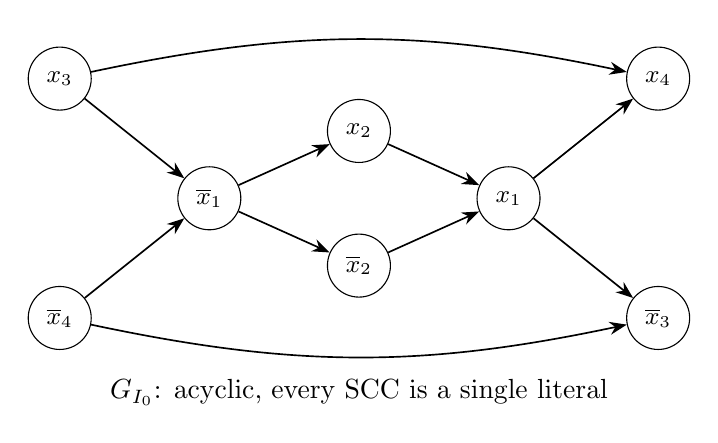
\begin{tikzpicture}[scale=0.95]
  \node[lit] (x3)  at (0, 1.6)  {$x_3$};
  \node[lit] (nx4) at (0,-1.6)  {$\neglit{x}_4$};
  \node[lit] (nx1) at (2, 0)    {$\neglit{x}_1$};
  \node[lit] (x2)  at (4, 0.9)  {$x_2$};
  \node[lit] (nx2) at (4,-0.9)  {$\neglit{x}_2$};
  \node[lit] (x1)  at (6, 0)    {$x_1$};
  \node[lit] (x4)  at (8, 1.6)  {$x_4$};
  \node[lit] (nx3) at (8,-1.6)  {$\neglit{x}_3$};
  \draw[imp] (x3) -- (nx1);  \draw[imp] (nx4) -- (nx1);
  \draw[imp] (nx1) -- (x2);  \draw[imp] (nx1) -- (nx2);
  \draw[imp] (x2) -- (x1);   \draw[imp] (nx2) -- (x1);
  \draw[imp] (x1) -- (x4);   \draw[imp] (x1) -- (nx3);
  \draw[imp] (x3) to[bend left=12] (x4);
  \draw[imp] (nx4) to[bend right=12] (nx3);
  \node at (4,-2.6) {$G_{I_0}$: acyclic, every SCC is a single literal};
\end{tikzpicture}
\hspace{1.2cm}
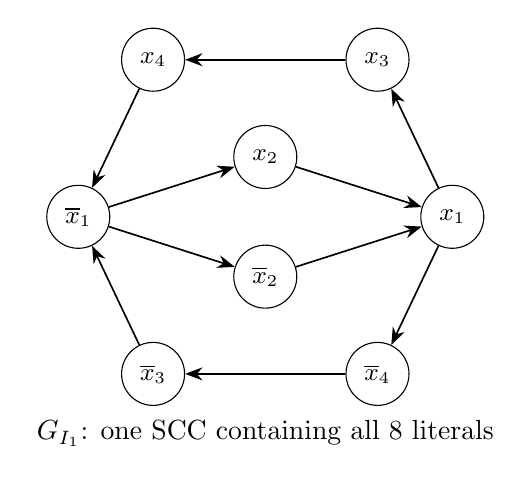
\begin{tikzpicture}[scale=0.95]
  \node[lit] (nx1) at (0, 0)    {$\neglit{x}_1$};
  \node[lit] (x2)  at (2.5, 0.8)  {$x_2$};
  \node[lit] (nx2) at (2.5,-0.8)  {$\neglit{x}_2$};
  \node[lit] (x1)  at (5, 0)    {$x_1$};
  \node[lit] (x3)  at (4, 2.1)  {$x_3$};
  \node[lit] (x4)  at (1, 2.1)  {$x_4$};
  \node[lit] (nx4) at (4,-2.1)  {$\neglit{x}_4$};
  \node[lit] (nx3) at (1,-2.1)  {$\neglit{x}_3$};
  \draw[imp] (nx1) -- (x2);  \draw[imp] (nx1) -- (nx2);
  \draw[imp] (x2) -- (x1);   \draw[imp] (nx2) -- (x1);
  \draw[imp] (x1) -- (x3);   \draw[imp] (x3) -- (x4);  \draw[imp] (x4) -- (nx1);
  \draw[imp] (x1) -- (nx4);  \draw[imp] (nx4) -- (nx3); \draw[imp] (nx3) -- (nx1);
  \node at (2.5,-2.9) {$G_{I_1}$: one SCC containing all $8$ literals};
\end{tikzpicture}
\end{center}

In $G_{I_0}$ no literal can reach itself (the left-to-right drawing is a topological order), so all eight SCCs are
singletons and no SCC contains both $x$ and $\neglit x$. In $G_{I_1}$,
$x_1\to x_3\to x_4\to\neglit{x}_1\to x_2\to x_1$, $\neglit{x}_1\to\neglit{x}_2\to x_1$ and
$x_1\to\neglit{x}_4\to\neglit{x}_3\to\neglit{x}_1$ are cycles through $x_1$ covering all eight literals, so they
form a single SCC, which contains $x_1$ and $\neglit{x}_1$.

\textbf{(d)}
\begin{lemma}[Edges are implications]
Under any satisfying assignment, if $\lambda\leadsto\mu$ is a path in $G_I$ and $\lambda$ is true, then $\mu$ is
true.
\end{lemma}
\begin{proof}
For a single edge $\neglit\alpha\to\beta$ coming from clause $(\alpha\vee\beta)$: if $\neglit\alpha$ is true then
$\alpha$ is false, so $\beta$ must be true for the clause to hold. The case of a path follows by induction on its
length.
\end{proof}
Suppose $x$ and $\neglit x$ lie in the same SCC, so there are paths $x\leadsto\neglit x$ and
$\neglit x\leadsto x$. In a satisfying assignment, if $x$ is true the first path makes $\neglit x$ true; if $x$ is
false then $\neglit x$ is true and the second path makes $x$ true. Both are contradictions, so $I$ is
unsatisfiable.

\textbf{(e)} Write $\neglit S=\{\neglit\lambda:\lambda\in S\}$ for a set of literals $S$.

\emph{Skew symmetry.} The edges $\neglit\alpha\to\beta$ and $\neglit\beta\to\alpha$ always come in pairs, so
$\lambda\to\mu$ is an edge iff $\neglit\mu\to\neglit\lambda$ is an edge; hence $\lambda\leadsto\mu$ iff
$\neglit\mu\leadsto\neglit\lambda$. Consequently, if $S$ is an SCC then so is $\neglit S$.

\emph{The procedure.} Let $R$ be the set of literals not yet deleted, initially all $2n$ of them. While
$R\neq\emptyset$: pick a sink SCC $S$ of the induced subgraph $G_I[R]$, make every literal of $S$ true and every
literal of $\neglit S$ false, and delete $S\cup\neglit S$ from $R$.

\emph{Invariant: $R$ is closed under negation and is a union of SCCs of $G_I$.} This holds initially. If it holds,
then the SCCs of $G_I[R]$ are exactly the SCCs of $G_I$ inside $R$ (a path between two vertices of one SCC $C$ of
$G_I$ stays inside $C\subseteq R$, and conversely mutual reachability in $G_I[R]$ implies it in $G_I$). So the
chosen $S$ is an SCC of $G_I$, $\neglit S$ is an SCC of $G_I$ by skew symmetry, and $\neglit S\subseteq R$ by
closure. Removing $S\cup\neglit S$ preserves both properties.

\emph{The assignment is well defined.} By hypothesis $S$ does not contain both $\lambda$ and $\neglit\lambda$, so
$S\cap\neglit S=\emptyset$ and no literal gets both values. Every step removes a variable together with its
negation, and assigns all of them, so at the end every variable has exactly one value.

\emph{No edge goes from a true literal to a false literal.} Suppose $\lambda\to\mu$ is an edge with $\lambda$ true
and $\mu$ false. Say $\lambda$ was assigned at step $t$ (so $\lambda\in S_t$) and $\mu$ at step $t'$
(so $\neglit\mu\in S_{t'}$).
\begin{itemize}[itemsep=0.2em]
\item If $t\le t'$: at the start of step $t$, $\mu$ is still in $R$. Since $S_t$ is a sink of $G_I[R]$ and
  $\lambda\in S_t$, the edge $\lambda\to\mu$ forces $\mu\in S_t$, so $\mu$ is true, a contradiction.
\item If $t'<t$: at the start of step $t'$, $\lambda$ and hence $\neglit\lambda$ are in $R$. The edge
  $\neglit\mu\to\neglit\lambda$ exists by skew symmetry and $\neglit\mu\in S_{t'}$, a sink, so
  $\neglit\lambda\in S_{t'}$ and $\lambda$ is false, a contradiction.
\end{itemize}

\emph{Every clause is satisfied.} Take a clause $(\alpha\vee\beta)$. If $\alpha$ were false, then $\neglit\alpha$
is true, and the edge $\neglit\alpha\to\beta$ forces $\beta$ to be true. So $I$ is satisfiable.

\textbf{(f)} By (d) and (e), $I$ is satisfiable iff no SCC of $G_I$ contains a variable together with its
negation. The algorithm:
\begin{enumerate}[itemsep=0.2em]
\item Build $G_I$: $2n$ vertices and $2m$ edges, in $O(n+m)$ time.
\item Compute its SCCs with the linear-time two-pass DFS algorithm, in $O(n+m)$ time, labelling each literal with
  its component.
\item For each variable $x$, compare the labels of $x$ and $\neglit x$ ($O(n)$ in total). If some pair agrees,
  output ``unsatisfiable''.
\item Otherwise output ``satisfiable''. A satisfying assignment can also be produced: that algorithm outputs the
  SCCs sink-first, i.e.\ each component it outputs is a sink of the graph left after removing the earlier ones.
  Process the components in that order and make the literals of a component true whenever they are still
  unassigned (and their negations false). Each component handled this way is a sink of a graph containing the
  current $G_I[R]$, hence a sink of $G_I[R]$, so this is an instance of the procedure in (e). It costs $O(n)$.
\end{enumerate}
The total running time is $O(n+m)$, linear in the size of the instance.

\end{document}
